% Options for packages loaded elsewhere
\PassOptionsToPackage{unicode}{hyperref}
\PassOptionsToPackage{hyphens}{url}
%
\documentclass[
]{article}
\usepackage{lmodern}
\usepackage{amssymb,amsmath}
\usepackage{ifxetex,ifluatex}
\ifnum 0\ifxetex 1\fi\ifluatex 1\fi=0 % if pdftex
  \usepackage[T1]{fontenc}
  \usepackage[utf8]{inputenc}
  \usepackage{textcomp} % provide euro and other symbols
\else % if luatex or xetex
  \usepackage{unicode-math}
  \defaultfontfeatures{Scale=MatchLowercase}
  \defaultfontfeatures[\rmfamily]{Ligatures=TeX,Scale=1}
\fi
% Use upquote if available, for straight quotes in verbatim environments
\IfFileExists{upquote.sty}{\usepackage{upquote}}{}
\IfFileExists{microtype.sty}{% use microtype if available
  \usepackage[]{microtype}
  \UseMicrotypeSet[protrusion]{basicmath} % disable protrusion for tt fonts
}{}
\makeatletter
\@ifundefined{KOMAClassName}{% if non-KOMA class
  \IfFileExists{parskip.sty}{%
    \usepackage{parskip}
  }{% else
    \setlength{\parindent}{0pt}
    \setlength{\parskip}{6pt plus 2pt minus 1pt}}
}{% if KOMA class
  \KOMAoptions{parskip=half}}
\makeatother
\usepackage{xcolor}
\IfFileExists{xurl.sty}{\usepackage{xurl}}{} % add URL line breaks if available
\IfFileExists{bookmark.sty}{\usepackage{bookmark}}{\usepackage{hyperref}}
\hypersetup{
  hidelinks,
  pdfcreator={LaTeX via pandoc}}
\urlstyle{same} % disable monospaced font for URLs
\usepackage[margin=1in]{geometry}
\usepackage{graphicx,grffile}
\makeatletter
\def\maxwidth{\ifdim\Gin@nat@width>\linewidth\linewidth\else\Gin@nat@width\fi}
\def\maxheight{\ifdim\Gin@nat@height>\textheight\textheight\else\Gin@nat@height\fi}
\makeatother
% Scale images if necessary, so that they will not overflow the page
% margins by default, and it is still possible to overwrite the defaults
% using explicit options in \includegraphics[width, height, ...]{}
\setkeys{Gin}{width=\maxwidth,height=\maxheight,keepaspectratio}
% Set default figure placement to htbp
\makeatletter
\def\fps@figure{htbp}
\makeatother
\setlength{\emergencystretch}{3em} % prevent overfull lines
\providecommand{\tightlist}{%
  \setlength{\itemsep}{0pt}\setlength{\parskip}{0pt}}
\setcounter{secnumdepth}{-\maxdimen} % remove section numbering
\usepackage{setspace}\doublespacing
\usepackage{lineno}\linenumbers

\author{}
\date{\vspace{-2.5em}}

\begin{document}

\hypertarget{a-standardized-effect-size-for-evaluating-the-strength-of-phylogenetic-signal-and-why-lambda-is-not-appropriate}{%
\section{A Standardized Effect Size for Evaluating the Strength of
Phylogenetic Signal, and Why Lambda is not
Appropriate}\label{a-standardized-effect-size-for-evaluating-the-strength-of-phylogenetic-signal-and-why-lambda-is-not-appropriate}}

\hfill\break

\textbf{Keywords}: phylogenetic signal, effect size, Pagel's lambda
\hfill\break

\textbf{Short Title}: An Effect Size for Phylogenetic Signal
\hfill\break

\hypertarget{abstract}{%
\section{Abstract}\label{abstract}}

\{conclusion holds: interpreting the regression is not appreciably
different (in terms of slopes and f values)\}

\newpage

\hypertarget{introduction}{%
\section{Introduction}\label{introduction}}

Investigating macroevolutionary patterns of trait variation requires a
phylogenetic perspective, because the shared ancestry among species
generates statistical non-independence (Felsenstein 1985; Harvey and
Pagel 1991). Accounting for this evolutionary non-independence is the
purview of \emph{phylogenetic comparative methods} (PCMs); a suite of
analytical tools that condition the data on the phylogeny through the
course of statisical evaluations of phenotypic trends (e.g., Grafen
1989; Garland and Ives 2000; Rohlf 2001; Butler and King 2004). The past
several decades have witnessed a rapid expansion in the development of
PCMs to address an ever-growing set of macroevolutionary hypotheses
(Martins and Hansen 1997; O'Meara et al. 2006; Revell and Harmon 2008;
Beaulieu et al. 2012; Adams 2014b,a; Adams and Collyer 2018). These
methods are predicated on the notion that phylogenetic signal -- the
tendancy for closely related species to display similar trait values --
is present in cross-species datasets (Felsenstein 1985; Pagel 1999;
Blomberg et al. 2003). Indeed, under numerous evolutionary models,
phylogenetic signal is to be expected, as stochastic character change
along the hierarchical structure of the tree of life generates trait
covaration among related taxa (see Felsenstein 1985; Blomberg et al.
2003; Revell et al. 2008). \hfill\break

Several analytical tools have been developed to quantify phylogenetic
signal in phenotypic datasets, including measures of serial independence
(\(\mathbf{C}\): Abouheif 1999), autocorrelation estimates (\(I\):
Gittleman and Kot 1990), statistical ratios of trait variation relative
to what is expected given the phylogeny (\(Kappa\): Blomberg et al.
2003; Adams 2014a), and scaling parameters used in maximum likelihood
fitting of the data to the phylogeny (\(\lambda\): Pagel 1999), among
others (e.g., Klingenberg and Gidaszewski 2010). The statistical
properties of these methods -- namely type I error rates and power --
have also been investigated to determine when phylogenetic signal can be
detected and under what conditions (e.g., Munkemuller et al. 2012;
Pavoine and Ricotta 2012; Diniz-Filho et al. 2012; Adams 2014a;
Molina-Venegas and Rodriguez 2017; see also Revell et al. 2008; Revell
2010). One of the most widely used methods for characterizing
phylogenetic signal in macroevolutionary studies is Pagel's \(\lambda\)
(Pagel 1999). Here, maximum likelihood is used to fit the data to the
phylogeny under a Brownian motion model of evolution. A parameter
(\(\lambda\)) is included, which transforms the lengths of the internal
branches of the phylogeny to improve the fit (Pagel 1999; Freckleton et
al. 2002). Pagel's \(\lambda\) ranges from \(0\to1\), with larger values
signifying a greater dependence of observed trait variation on the
phylogeny. Pagel's \(\lambda\) also has the appeal that it may be
included in phylogenetic regression (PGLS) to account for the degree of
phylogenetic signal in comparative analyses (see Freckleton et al.
2002). \hfill\break

Evolutionary biologists commonly seek to describe the relative strength
of phylogenetic signal in phenotypic traits, to determine the extent to
which shared evolutionary history has influenced trait covariation among
taxa. This is often accomplished by interpreting empirical estimates of
\(\lambda\); with smaller values signifying `weak' phylogenetic signal,
while larger values are interpreted as `strong' phylogenetic signal
(e.g., De Meester et al. 2019; Pintanel et al. 2019; Su et al. 2019).
Other approaches for interpreting \(\lambda\) are more statistical. For
instance, some have evaluated whether the observed \(\lambda\) differs
from some expected value through the use of confidence intervals
(Vandelook et al. 2019) or by performing likelihood ratio tests that
compare the observed model fit to that obtained when \(\lambda=0\) or
\(\lambda=1\) (Freckleton et al. 2002; Cooper et al. 2010; Bose et al.
2019). Additionally, qualitative comparisons of \(\lambda\) estimates
obtained from multiple phenotypic traits have been used to infer whether
the strength of phylogenetic signal is greater in one trait as compared
to another (e.g., Liu et al. 2019; Bai et al. 2019). Indeed, statements
regarding the strength of phylogenetic signal based on \(\lambda\) are
rather common in the evolutionary literature. We conducted a literature
survey in Google.scholar and found that of the 204 papers published in
2019 that estimated and reported Pagel's \(\lambda\), 40\% interpreted
the strength of phylogenetic signal for at least one phenotypic trait.
Additionally, nearly 30\% of the 421 \(\lambda\) estimates between 0.25
and 0.75 were assigned a strength of signal, and because nearly half of
the 1,572 values reported were near the limits of the parameter (Figure
1), this percentage is even higher, as biological interpretation of
phylogenetic signal at the limits of \(\lambda\) are known. \hfill\break

{[}insert Figure 1 here{]} \hfill\break

It seems intuitive to interpret the strength of phylogenetic signal
based on the value of \(\lambda\), as \(\lambda\) is a parameter on a
bounded scale (\(0\to1\)) for which interpretation of its extremal
points are understood. Specifically, \(\lambda=0\) represents no
phylogenetic signal, while \(\lambda=1\) is phylogenetic signal as
expected under Brownian motion. However, equating values of \(\lambda\)
directly to the strength of phylogenetic signal presumes two important
statistical properties that have not been fully explored. First, it
presumes that values of \(\lambda\) can be precisely estimated, as
biological inferences regarding the strength of phylogenetic signal
depend on high accuracy in its estimation. Therefore, understanding the
precision in estimating \(\lambda\) is paramount. One study (Boettiger
et al. 2012) found that estimates of Pagel's \(\lambda\) displayed less
variation (i.e., greater precision) when data were simulated on a large
phylogeny (\(N=281\)) as compared to a small one (\(N=13\)). From this
observation it was concluded that insufficient data (i.e., the number of
species) was the underlying cause of the increased variation across
parameter estimates (Boettiger et al. 2012). Indeed, such a pattern is
common with statistical estimators, as summary statistics and parameters
are often more precise at greater sample sizes (Cohen 1988). However,
this conclusion also assumes that the precision of \(\lambda\) remains
constant across its range (\(\lambda = 0 \to 1\)); an assumption that to
date, has not been verified. Thus, despite widespread use of Pagel's
(1999) \(\lambda\) in macroevolutionary studies, at present, we still
lack a general understanding of the precision with which \(\lambda\) can
estimate levels of phylogenetic signal in phenotypic datasets.
\hfill\break

Second, while estimates of \(\lambda\) are within a bounded scale
(\(0\to1\)), this does not \emph{de-facto} imply that the estimated
values of this parameter correspond to the actual strength of the
underlying input signal in the data. For this to be the case,
\(\lambda\) must be a statistical effect size. Effect sizes are a
measure the magnitude of a statistical effect in data, represented on a
common scale (Glass 1976; Cohen 1988). Effect sizes have widespread use
in many areas of the quantiative sciences, as they represent measures
that may be readily summarized across datasets as in meta-analysis
(Glass 1976; Hedges and Olkin 1985; Arnqvist and Wooster 1995), or
compared among datasets (e.g., Adams and Collyer 2016, 2019a).
Unfortunatley, not all model parameters and test statistics are effect
sizes, and thus many summary measures must first be converted to
standardized units (i.e., an effect size) for meaningful comparison (see
Rosenthal 1994). As a consequence, it follows that only if \(\lambda\)
is a statistical effect size can comparisons of estimates across
datasets be interpretable. For the case of \(\lambda\), this has not yet
been explored. \hfill\break

In this study, we evaluate the precision of Pagel's \(\lambda\) in
estimating known levels of phylogenetic signal in phenotypic data. We
use computer simulations with differing numbers of species, differently
shaped phylogenies, and differing input levels of phylogenetic signal,
to explore the degree to which \(\lambda\) correctly identifies known
levels of phylogenetic signal, and under what circumstances. We find
that while PGLS parameters (e.g., \(\beta\)) are accurately estimated
with the inclusion of phylogenetic signal, estimates of \(\lambda\) are
not. We also find that estimates of \(\lambda\) vary widely for a given
input value of phylogenetic signal, and that the precision in estimating
\(\lambda\) is not constant across the range of input signal, with
decreased precision when phylogenetic signal is of intermediate
strength. Additionally, the same \(\lambda_{est}\) may be obtained from
datasets containing vastly different input levels of phylogenetic
signal. Thus, \(\lambda\) is not a reliable estimate of the strength of
phylogenetic signal in phenotypic data. We subsequently derive a
standardized effect size for measuring the strength of phylogenetic
signal in phenotypic datasets, and apply the concept to two common
measures of phylogenetic signal: \(\lambda\) and \(Kappa\). Through
simulations across a wide range of conditions, we find that the
precision of effect sizes based on \(\lambda\) (\(Z_{\lambda}\)) are
less reliable than that those based on \(Kappa\) (\(Z_K\)), implying
that \(Z_K\) is a more robust effect size measure. Additionally, we
propose a two-sample test statistic that may be used to compare the
strength of phylogenetic signal among datasets, and provide an empirical
example to demonstrate its use. We conclude that estimates of
phylogenetic signal using Pagel's \(\lambda\) are often inaccurate, and
thus interpreting strength of phylogenetic signal in phenotypic datasets
based on this measure is compromised. By contrast, effect sizes obtained
from \(Kappa\) hold promise for characterizing phylogenetic signal, and
for comparing the strength of phylogenetic signal across datasets.

\hypertarget{methods-and-results}{%
\section{Methods and Results}\label{methods-and-results}}

\hypertarget{the-precision-of-lambda-is-variable}{%
\subsection{\texorpdfstring{\emph{The Precision of \(\lambda\) is
Variable}}{The Precision of \textbackslash lambda is Variable}}\label{the-precision-of-lambda-is-variable}}

We conducted a series of computer simulations to evaluate the precision
of Pagel's \(\lambda\). Our primary simulations were based on pure-birth
phylogenies; however, we also evaluated patterns on both balanced and
pectinate trees to determine whether tree shape affected our findings
(see Supporting Information). First we generated 50 pure-birth
phylogenies at each of six different tree sizes, ranging from 32 to 1024
taxa (\(n=2^5 - 2^{10}\)). Next, we rescaled the simulated phylogenies
by multiplying the internal branches by \(\lambda_{in}\), using 21
intervals of 0.05 units across its range
(\(\lambda_{in} = 0.0 \to 1.0\)), resulting in 1050 scaled phylogenies
at each level of species richness (\(n\)). Continuous traits were then
simulated on each phylogeny under a Brownian motion model of evolution
to obtain datasets with differing levels of phylogenetic signal, that
ranged from no phylogenetic signal (when \(\lambda_{in} =0\)), to
phylogenetic signal corresponding reflecting Brownian motion (when
\(\lambda_{in} =1\)). For each dataset we then estimated phylogenetic
signal (\(\lambda_{est}\)), and calculated the precision of \(\lambda\)
using the variance (\(\sigma^2_\lambda\)) across datasets at each input
level of phylogenetic signal and level of species richness. \hfill\break

We also evaluated the precision of \(\lambda\) when estimated in PGLS
regression and ANOVA (i.e., \(Y\sim{X}\)). Here, an independent variable
\(X\) was simulated on each phylogeny under a Brownian motion model of
evolution (for PGLS regression). For phylogenetic ANOVA, random groups
(\(X\)) were obtained by simulating a discrete (binary) character on
each phylogeny. Next, the dependent variable was simulated in such a
manner as to contain a known relationship with \(X\) plus random error
containing phylogenetic signal. This was accomplished as:
\(Y=\beta{X}+\epsilon\). Here, the association between \(Y\) and \(X\)
was modeled using a range of values:
\(\beta=(0.0,0.25, 0.5, 0.75,1.0)\), and the residual error was modeled
to contain phylogenetic signal simulated under a Brownian motion model
of evolution: \(\epsilon=\mathcal{N}(\mu=0,\sigma=\mathbf{C})\): (see
Revell 2010 for a similar simulation design). The fit of the
phylogenetic regression was estimated using maximum likelihood, and
parameter estimates (\(\beta_{est}\) and \(\lambda_{est}\)) were
obtained. Precision estimates (\(\sigma^2_\lambda\)) at each input level
of phylogenetic signal and level of species richness were then observed.
\hfill\break

All analyses were performed in R v3.6.0 (R Core Team 2019) using the
packages \texttt{geiger} (Harmon et al. 2008), \texttt{caper} (Orme et
al. 2013), \texttt{phytools} (Revell 2012), and \texttt{geomorph} (Adams
and Otárola-Castillo 2013; Adams et al. 2020). R-scripts are found in
the Supporting Information. \hfill\break

\emph{Results.} We found that the precision of \(\lambda_{est}\) varied
widely across simulation conditions. Predictably, precision improved as
the number of species increased (Figure 2). This confirmed earlier
findings of Boettiger et al.~(2012), and adhered to parametric
statistical theory. However, in many cases the set of \(\lambda_{est}\)
spanned nearly the entire range of possible values (e.g., \(n=32\);
\(\lambda_{in}=0.5\): \(\lambda_{est}= 0.0\to 0.985\)), revealing that
estimates of \(\lambda\) were not a reliable indicator of input
phylogenetic signal. Importantly, the precision of \(\lambda_{est}\) was
not uniform across all levels of phylogenetic signal, with the worst
precision at intermediate levels of signal (\(\lambda_{in}\approx0.5\)),
and improved precision as input levels approached the extremes of its
range (i.e., \(\lambda_{in}\rightarrow0\) \&
\(\lambda_{in}\rightarrow1\)). Thus, estimates of \(\lambda\) were least
reflective of the true input signal at intermediate values.
Additionally, even at large levels of species richness, we found that
the range of \(\lambda_{est}\) still encompassed a substantial portion
of possible values (e.g., \(n=512\); \(\lambda_{in}=0.5\):
\(\lambda_{est} = 0.32\to 0.68\)). Likewise, the same \(\lambda_{est}\)
could be obtained from datasets containing vastly different input levels
of phylogenetic signal (e.g., \(n=512\); \(\lambda_{est} = 0.5\);
\(\lambda_{in} = 0.25 \to 0.65\)). Results were similar when \(\lambda\)
was co-estimated with regression parameters in PGLS regression (Figure
3). Here, regression parameters (\(\beta\)) were accurately estimated,
confirming earlier findings of Revell 2010 (2010) (see Supporting
Information). However, estimates of phylogenetic signal were not, and
the spread of \(\lambda_{est}\) was even broader than that observed when
\(\lambda\) was estimated for only the dependent variable. Taken
together, these findings reveal that \(\lambda_{est}\) does not
precisely characterize observed levels of phylogenetic signal in
phenotypic datasets, and that biological interpretations of the strength
of phylogenetic signal based on \(\lambda\) may be highly inaccurate.
\hfill\break

{[}insert Figure 2 here{]} \hfill\break

{[}insert Figure 3 here{]} \hfill\break 

\hypertarget{a-standardized-effect-size-for-phylogenetic-signal}{%
\subsection{\texorpdfstring{\emph{A Standardized Effect Size for
Phylogenetic
Signal}}{A Standardized Effect Size for Phylogenetic Signal}}\label{a-standardized-effect-size-for-phylogenetic-signal}}

The results above demonstate that \(\lambda\) is not a reliable estimate
of the phylogenetic signal in phenotypic data. As such, biological
interpretations of the strength of phylogenetic signal, and comparisons
of the magnitude of such effects across datasets, are severely
compromised when based on this parameter. As an alternative, we propose
that summary estimates of phylogenetic signal be converted to effect
sizes for interpretation and comparison. Statistically, a standardized
effect size may be found as:

\begin{align}
    Z_{\theta}=\frac{\theta_{obs}-E(\theta)}{\sigma_\theta}
\end{align}

where \(\theta_{obs}\) is the observed test statistic, \(E(\theta)\) is
its expected value under the null hypothesis, and \(\sigma_\theta\) is
its standard error (Glass 1976; Cohen 1988; Rosenthal 1994).
\(Z_{\theta}\) expresses the magnitude of the effect in \(\theta_{obs}\)
by transforming the original test statistic to a standard normal deviate
(Glass 1976; Kelley and Preacher 2012). Typically, \(\theta_{obs}\) and
\(\sigma_\theta\) are estimated from the data, while \(E(\theta)\) is
obtained from the distribution of \(\theta\) derived from parametric
theory. However, recent advances in resampling theory (Collyer et al.
2015; Adams and Collyer 2016, 2019a) have shown that \(E(\theta)\) and
\(\sigma_\theta\) may also be obtained from an empirical sampling
distribution of \(\theta\) obtained from permutation procedures.
\hfill\break

Adams and Collyer (2019b) recently suggested that the strength of
phylogenetic signal could be represented as an effect size, based on the
\(Kappa\) statistic and its empirical sampling distribution from
permutation. Here we formalize that suggestion, and find an effect size
as:

\begin{align}
    Z_{K}=\frac{K_{obs}-\hat\mu_K}{\hat\sigma_K}
\end{align}

where \(K_{obs}\) is the observed phylogenetic signal, and \(\hat\mu_K\)
and \(\hat\sigma_K\) are the mean and standard deviation of the
empirical sampling distribution of \(Kappa\) obtained via permutation.
Similarly, an effect size based on \(\lambda\) could be envisioned as:

\begin{align}
    Z_{\lambda}=\frac{\lambda_{obs}-0}{\hat\sigma_\lambda}.
\end{align}

In this case, \(\lambda_{obs}\) and \(\hat\sigma_\lambda\) are
empirically derived using maximum likelihood. Note also that under the
null hypothesis, \(E(\lambda)=0\), a no phylogenetic signal is expected
under this condition (Freckleton et al. 2002). \hfill\break

To evaluate the utility of \(Z_K\) and \(Z_\lambda\) we calculated both
effect sizes for the simulated datasets generated above, and summarized
the precision of each using its variance (\(\sigma^2_{Z_K}\) and
\(\sigma^2_{Z_\lambda}\)). Results are found in Figure 4. Here two
things are evident. First, estimates of \(Z_K\) track the input
phylogenetic signal in a more linear fashion than do estimates of
\(Z_\lambda\). Second, the precision of \(Z_K\) is considerably more
stable as compared with \(Z_\lambda\), as coefficients of variation for
the set of \(\sigma^2_{Z_K}\) across input levels of phylogenetic signal
were an order of magnitude smaller for than was observed for
\(\sigma^2_{Z_\lambda}\) (Figure 4). This implied that estimates of the
strength of phylogenetic signal were more reliable and robust when using
\(Z_K\) as compared with \(Z_\lambda\). \hfill\break

{[}insert Figure 4 here{]}

\hypertarget{statistical-comparisons-of-phylogenetic-signal}{%
\subsection{\texorpdfstring{\emph{Statistical Comparisons of
Phylogenetic
Signal}}{Statistical Comparisons of Phylogenetic Signal}}\label{statistical-comparisons-of-phylogenetic-signal}}

Once the magnitude of phylogenetic signal is characterized using
\(Z_K\), it may be of interest to compare such measures across datasets.
This is useful, for instance, to determine whether the strength of
phylogenetic signal is greater in one phenotypic trait as compared with
another. As with other effect sizes derived from permutation
distributions (e.g., Adams and Collyer 2016, 2019a), a two-sample test
statistic may be found as:

\begin{align}
  \hat{Z}_{12}=\frac{\lvert{(K_{1}-\hat\mu_{K_1})-(K_{2}-\hat\mu_{K_2})}\rvert}{\sqrt{\hat\sigma^2_{K_1}+\hat\sigma^2_{K_2}}}
\end{align}

where \(K_1\), \(K_2\), \(\hat\mu_{K_1}\), \(\hat\mu_{K_2}\),
\(\hat\sigma_{K_1}\), and \(\hat\sigma_{K_2}\) are as defined above for
equation 2. Estimates of significance of \(\hat{Z}_{12}\) may be
obtained from a standard normal distribution. As with other two-sample
tests, \(\hat{Z}_{12}\) is typically considered a two-tailed test,
however directional (one-tailed) tests may be specified should the
empirical situation require it (see Adams and Collyer 2016, 2019a).

\hypertarget{empirical-example}{%
\subsection{\texorpdfstring{\emph{Empirical
Example}}{Empirical Example}}\label{empirical-example}}

\hypertarget{conclusions-and-implications}{%
\section{Conclusions and
Implications}\label{conclusions-and-implications}}

1: summary paragraph

2: expand on Lambda.. lambda innacurate, not precise, level of precision
varies with input physig (worse in mid-range). NEW RESULT. We are first
to show this. NOTE: pattern is obvious with reflection. Since it is a
`bounded' parameter estimation should be best at the extremes\ldots{}
(state this?).. hmm.

Patterns worse with PGLS, though beta still estimated properly.
Conclusion, lambda not overly useful.

3: By contrast, effect size Z-K useful, equally precise across range of
values. Can be used to characterize the strength of physignal, and
because robust to input levels, etc. may be used to compare across
datasets.

Somewhere, recognize that this is somewhat `backwards' from prior
recommendations where Kappa had somewhat lower performance in terms of
type I and type II error (which?? I forget). However, recall that those
studies did not examine the precision of the estimates. Nor was Z-k
included, because it was not yet invented. So Use of Z-k should make
good sense here.

Closing paragraph.

\hfill\break

More discussion paragraphs

\newpage

\hypertarget{references}{%
\section{References}\label{references}}

\setlength{\parindent}{-0.25in} \setlength{\leftskip}{0.25in}
\setlength{\parskip}{8pt} \noindent

\hypertarget{refs}{}
\leavevmode\hypertarget{ref-Abouheif1999}{}%
Abouheif, E. 1999. A method for testing the assumption of phylogenetic
independence in comparative data. Evolutionary Ecology Research
1:895--909.

\leavevmode\hypertarget{ref-Adams2014a}{}%
Adams, D. C. 2014a. A generalized Kappa statistic for estimating
phylogenetic signal from shape and other high-dimensional dultivariate
data. Systematic Biology 63:685--697.

\leavevmode\hypertarget{ref-Adams2014b}{}%
Adams, D. C. 2014b. A method for assessing phylogenetic least squares
models for shape and other high-dimensional multivariate data. Evolution
68:2675--2688.

\leavevmode\hypertarget{ref-AdamsCollyer2019b}{}%
Adams, D. C., and M. L. Collyer. 2019a. Comparing the strength of
modular signal, and evaluating alternative modular hypotheses, using
covariance ratio effect sizes with morphometric data. Evolution
73:2352--2367.

\leavevmode\hypertarget{ref-AdamsCollyer2016}{}%
Adams, D. C., and M. L. Collyer. 2016. On the comparison of the strength
of morphological integration across morphometric datasets. Evolution
70:2623--2631.

\leavevmode\hypertarget{ref-AdamsCollyer2018b}{}%
Adams, D. C., and M. L. Collyer. 2018. Phylogenetic anova: Group-clade
aggregation, biological challenges, and a refined permutation procedure.
Evolution 72:1204--1215.

\leavevmode\hypertarget{ref-AdamsCollyer2019}{}%
Adams, D. C., and M. L. Collyer. 2019b. Phylogenetic comparative methods
and the evolution of multivariate phenotypes. Annual Review of Ecology,
Evolution, and Systematics 50:405--425.

\leavevmode\hypertarget{ref-AdamsGeomorph}{}%
Adams, D. C., M. L. Collyer, and A. Kaliontzopoulou. 2020. Geomorph:
Software for geometric morphometric analyses. R package version 3.2.1.

\leavevmode\hypertarget{ref-AdamsOtarola2013}{}%
Adams, D. C., and E. Otárola-Castillo. 2013. Geomorph: An r package for
the collection and analysis of geometric morphometric shape data.
Methods in Ecology and Evolution 4:393--399.

\leavevmode\hypertarget{ref-Arnqvist1995}{}%
Arnqvist, G., and D. Wooster. 1995. Meta-analysis: Synthesizing research
findings in ecology and evolution. Trends in Ecology and Evolution
10:236--240.

\leavevmode\hypertarget{ref-Bai2019}{}%
Bai, K., S. Lv, S. Ning, D. Zeng, Y. Guo, and B. Wang. 2019. Leaf
nutrient concentrations associated with phylogeny, leaf habit and soil
chemistry in tropical karst seasonal rainforest tree species. Plant and
Soil 434:305--326.

\leavevmode\hypertarget{ref-Beaulieu_et_al2012}{}%
Beaulieu, J. M., D. C. Jhwueng, C. Boettiger, and B. C. O'Meara. 2012.
Modeling stabilizing selection: Expanding the ornstein-uhlenbeck model
of adaptive evolution. Evolution 66:2369--2383.

\leavevmode\hypertarget{ref-Blomberg_et_al2003}{}%
Blomberg, S. P., T. Garland, and A. R. Ives. 2003. Testing for
phylogenetic signal in comparative data: Behavioral traits are more
labile. Evolution 57:717--745.

\leavevmode\hypertarget{ref-Boettiger_et_al2012}{}%
Boettiger, C., G. Coop, and P. Ralph. 2012. Is your phylogeny
informative? Measuring the power of comparative methods. Evolution
67:2240--2251.

\leavevmode\hypertarget{ref-Bose2019}{}%
Bose, R., B. R. Ramesh, R. Pélissier, and F. Munoz. 2019. Phylogenetic
diversity in the western ghats biodiversity hotspot reflects
environmental filtering and past niche diversification of trees. Journal
of Biogeography 46:145--157.

\leavevmode\hypertarget{ref-ButlerKing2004}{}%
Butler, M. A., and A. A. King. 2004. Phylogenetic comparative analysis:
A modeling approach for adaptive evolution. American Naturalist
164:683--695.

\leavevmode\hypertarget{ref-Cohen1988}{}%
Cohen, J. 1988. Statistical power analysis for the behavioral sciences.
Routledge.

\leavevmode\hypertarget{ref-Collyer_et_al2015a}{}%
Collyer, M. L., D. J. Sekora, and D. C. Adams. 2015. A method for
analysis of phenotypic change for phenotypes described by
high-dimensional data. Heredity 115:357--365.

\leavevmode\hypertarget{ref-Cooper2010}{}%
Cooper, N., W. Jetz, and R. P. Freckleton. 2010. Phylogenetic
comparative approaches for studying niche conservatism. Journal of
Evolutionary Biology 23:2529--2539.

\leavevmode\hypertarget{ref-DeMeester2019}{}%
De Meester, G., K. Huyghe, and R. Van Damme. 2019. Brain size, ecology
and sociality: A reptilian perspective. Biological Journal of the
Linnean Society 126:381--391.

\leavevmode\hypertarget{ref-DinizFilho2012}{}%
Diniz-Filho, J. A. F., T. Santos, T. F. Rangel, and L. M. Bini. 2012. A
comparison of metrics for estimating phylogenetic signal under
alternative evolutionary models. Genetics and Molecular Biology
35:673--679.

\leavevmode\hypertarget{ref-Felsenstein1985}{}%
Felsenstein, J. 1985. Phylogenies and the comparative method. American
Naturalist 125:1--15.

\leavevmode\hypertarget{ref-Freckleton_et_al2002}{}%
Freckleton, R. P., P. H. Harvey, and M. Pagel. 2002. Phylogenetic
analysis and comparative data: A test and review of evidence. American
Naturalist 160:712--726.

\leavevmode\hypertarget{ref-GarlandIves2000}{}%
Garland, T. J., and A. R. Ives. 2000. Using the past to predict the
present: Confidence intervals for regression equations in phylogenetic
comparative methods. American Naturalist 155:346--364.

\leavevmode\hypertarget{ref-Gittleman1990}{}%
Gittleman, J. L., and M. Kot. 1990. Adaptation: Statistics and a null
model for estimating phylogenetic effects. Systematic Zoology
39:227--241.

\leavevmode\hypertarget{ref-Glass1976}{}%
Glass, G. V. 1976. Primary, secondary, and meta-analysis of research.
Educational Researcher 5:3--8.

\leavevmode\hypertarget{ref-Grafen1989}{}%
Grafen, A. 1989. The phylogenetic regression. Philosophical Transactions
of the Royal Society of London B, Biological Sciences 326:119--157.

\leavevmode\hypertarget{ref-Harmon2008}{}%
Harmon, L. J., J. T. Weir, C. D. Brock, R. E. Glor, and W. Challenger.
2008. GEIGER: Investigating evolutionary radiations. Bioinformatics
24:129--131.

\leavevmode\hypertarget{ref-HarveyPagel1991}{}%
Harvey, P. H., and M. D. Pagel. 1991. The comparative method in
evolutionary biology. Oxford University Press, Oxford.

\leavevmode\hypertarget{ref-HedgesOlkin1985}{}%
Hedges, L. V., and I. Olkin. 1985. Statistical methods for
meta-analysis. Elsevier.

\leavevmode\hypertarget{ref-Kelley2012}{}%
Kelley, K., and K. J. Preacher. 2012. On effect size. Psychological
Methods 17:137--152.

\leavevmode\hypertarget{ref-Klingenberg2010}{}%
Klingenberg, C. P., and N. A. Gidaszewski. 2010. Testing and quantifying
phylogenetic signals and homoplasy in morphometric data. Systematic
biology 59:245--261.

\leavevmode\hypertarget{ref-Liu2019}{}%
Liu, H., C. P. Osborne, D. Yin, R. P. Freckleton, G. Jiang, and M. Liu.
2019. Phylogeny and ecological processes influence grass coexistence at
different spatial scales within the steppe biome. Oecologia 191:25--38.

\leavevmode\hypertarget{ref-MartinsHansen1997}{}%
Martins, E. P., and T. F. Hansen. 1997. Phylogenies and the comparative
method: A general approach to incorporating phylogenetic information
into the analysis of interspecific data. American Naturalist
149:646--667.

\leavevmode\hypertarget{ref-MolinaVenegas2017}{}%
Molina-Venegas, R., and M. A. Rodriguez. 2017. Revisiting phylogenetic
signal; strong or negligible impacts of polytomies and branch length
information? BMC evolutionary biology 17:53.

\leavevmode\hypertarget{ref-Munkemuller_et_al2012}{}%
Munkemuller, T., S. Lavergne, B. Bzeznik, S. Dray, T. Jombart, K.
Schiffers, and W. Thuiller. 2012. How to measure and test phylogenetic
signal. Methods in Ecology and Evolution 3:743--756.

\leavevmode\hypertarget{ref-OMeara_et_al2006}{}%
O'Meara, B. C., C. Ane, M. J. Sanderson, and P. C. Wainwright. 2006.
Testing for different rates of continuous trait evolution using
likelihood. Evolution 60:922--933.

\leavevmode\hypertarget{ref-Orme2013}{}%
Orme, D., R. P. Freckleton, G. H. Thomas, T. Petzoldt, S. A. Fritz, and
N. Isaac. 2013. CAPER: Comparative analyses of phylogenetics and
evolution in r. Methods in Ecology and Evolution 3:145--151.

\leavevmode\hypertarget{ref-Pagel1999}{}%
Pagel, M. D. 1999. Inferring the historical patterns of biological
evolution. Nature 401:877--884.

\leavevmode\hypertarget{ref-Pavoine2012}{}%
Pavoine, S., and C. Ricotta. 2012. Testing for phylogenetic signal in
biological traits: The ubiquity of cross-product statistics. Evolution:
International Journal of Organic Evolution 67:828--840.

\leavevmode\hypertarget{ref-Pintanel2019}{}%
Pintanel, P., M. Tejedo, S. R. Ron, G. A. Llorente, and A.
Merino-Viteri. 2019. Elevational and microclimatic drivers of thermal
tolerance in andean pristimantis frogs. Journal of Biogeography
46:1664--1675.

\leavevmode\hypertarget{ref-RCT}{}%
R Core Team. 2019. R: A language and environment for statistical
computing. R Foundation for Statistical Computing, Vienna, Austria.

\leavevmode\hypertarget{ref-Revell2010}{}%
Revell, L. J. 2010. Phylogenetic signal and linear regression on species
data. Methods in Ecology and Evolution 1:319--329.

\leavevmode\hypertarget{ref-Revell2012}{}%
Revell, L. J. 2012. Phytools: An r package for phylogenetic comparative
biology (and other things). Methods in Ecology and Evolution 3:217--223.

\leavevmode\hypertarget{ref-RevellHarmon2008}{}%
Revell, L. J., and L. J. Harmon. 2008. Testing quantitative genetic
hypotheses about the evolutionary rate matrix for continuous characters.
Evolutionary Ecology Research 10:311--331.

\leavevmode\hypertarget{ref-Revell_et_al2008}{}%
Revell, L. J., L. J. Harmon, and D. C. Collar. 2008. Phylogenetic
signal, evolutionary process, and rate. Systematic Biology 57:591--601.

\leavevmode\hypertarget{ref-Rohlf2001}{}%
Rohlf, F. J. 2001. Comparative methods for the analysis of continuous
variables: Geometric interpretations. Evolution 55:2143--2160.

\leavevmode\hypertarget{ref-Rosenthal1994}{}%
Rosenthal, R. 1994. The handbook of research synthesis. Pp. 231--244
\emph{in} L. V. Cooper H Hedges, ed. Russell Sage Foundation.

\leavevmode\hypertarget{ref-Su2019}{}%
Su, G., S. Villéger, and S. Brosse. 2019. Morphological diversity of
freshwater fishes differs between realms, but morphologically extreme
species are widespread. Global ecology and biogeography 28:211--221.

\leavevmode\hypertarget{ref-Vandelook2019}{}%
Vandelook, F., S. Janssens, P. Gijbels, E. Fischer, W. Van den Ende, O.
Honnay, and S. Abrahamczyk. 2019. Nectar traits differ between
pollination syndromes in balsaminaceae. Annals of Botany 124:269--279.

\newpage

\hypertarget{figure-legends}{%
\section{Figure Legends}\label{figure-legends}}

\textbf{Figure 1}. Frequency distribution of \(\lambda\) estimates
published in 2019. The majority of these values were close to 0 or 1,
and from phylogenies with fewer than 200 taxa. \hfill\break

\textbf{Figure 2}. Precision of Pagel's \(\lambda\) across known levels
of input phylogenetic signal (\(\lambda_{in}\)) on phylogenies of
various sizes. As phylogenies increase in size, variation in
\(\lambda_{in}\) decreases; however the precision is not constant across
the range of input levels (\(\lambda_{in}: 0 \to 1\)), and is highest at
intermediate levels of phylogenetic signal. \hfill\break

\textbf{Figure 3}. Precision of Pagel's \(\lambda\) when incorporated in
phylogenetic regression (\(Y\sim X\)), across known levels of input
phylogenetic signal (\(\lambda_{in}\)) on phylogenies of various sizes.
As phylogenies increase in size, variation in \(\lambda_{in}\)
decreases; however the precision is not constant across the range of
input levels (\(\lambda_{in}: 0 \to 1\)), and is highest at intermediate
levels of phylogenetic signal. \hfill\break

\textbf{Figure 4}. Variation in estimates of phylogenetic signal across
input levels of phylogenetic signal. (A) Estimates of Pagel's
\(\lambda\) for data simulated on phylogenies with 128 taxa (\(n=128\)),
(B) Estimates of \(Z_K\) for data simulated on phylogenies with 128 taxa
(\(n=128\)), (C) Variance in the variation of \(\lambda_{est}\) across
input levels of phylogenetic signal, estimated on phylogenies containing
differing numbers of species. (D) Variance in the variation of \(Z_K\)
across input levels of phylogenetic signal, estimated on phylogenies
containing differing numbers of species.

\newpage

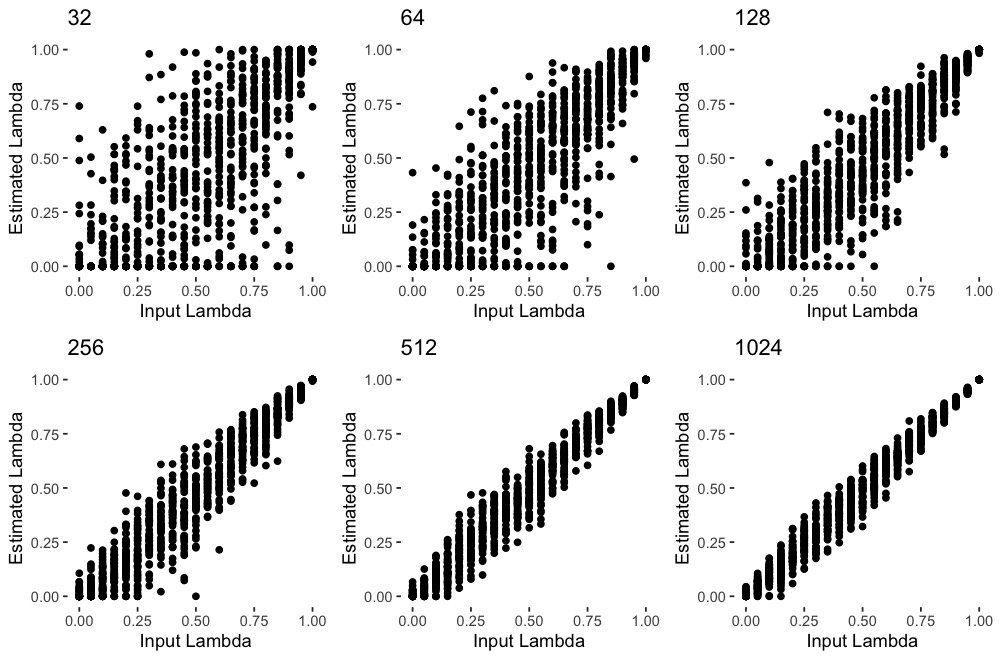
\includegraphics[width=0.95\linewidth]{Fig1}

\singlespacing \textbf{Figure 1}. Frequency distribution of \(\lambda\)
estimates published in 2019. The majority of these values were close to
0 or 1, and from phylogenies with fewer than 200 taxa.

\newpage

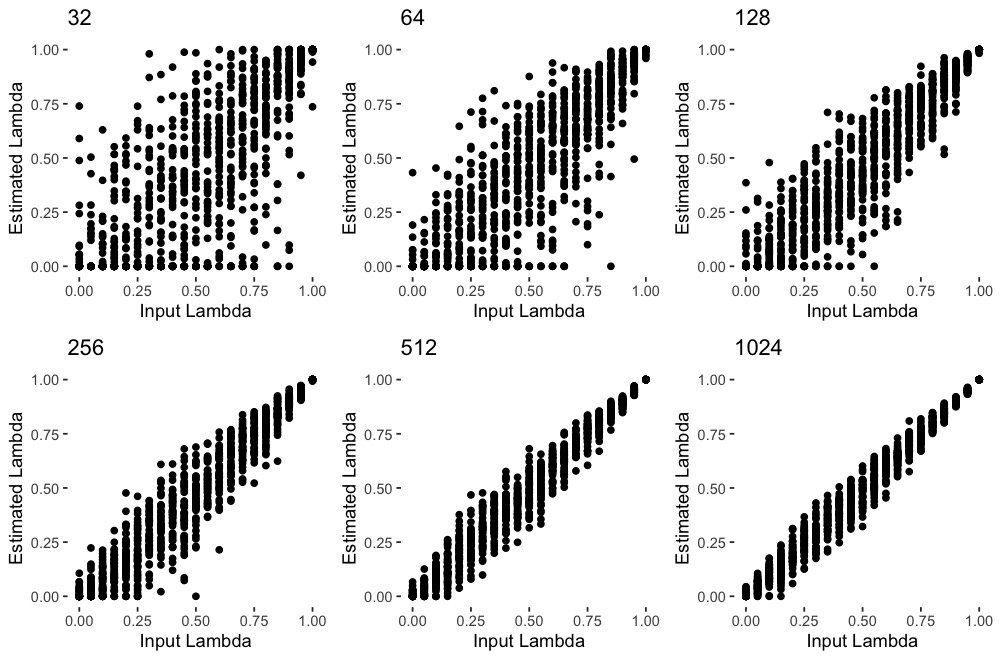
\includegraphics[width=0.95\linewidth]{Fig2}

\singlespacing \textbf{Figure 2}. Precision of Pagel's \(\lambda\)
across known levels of input phylogenetic signal (\(\lambda_{in}\)) on
phylogenies of various sizes. As phylogenies increase in size, variation
in \(\lambda_{in}\) decreases; however the precision is not constant
across the range of input levels (\(\lambda_{in}: 0 \to 1\)), and is
highest at intermediate levels of phylogenetic signal.

\newpage

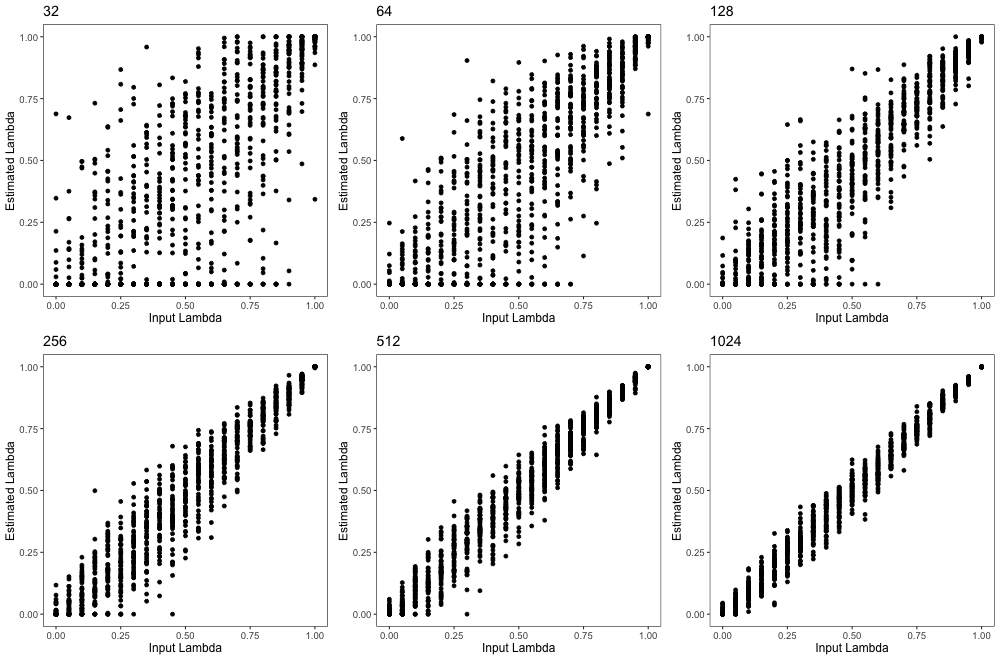
\includegraphics[width=0.95\linewidth]{Fig3}

\singlespacing \textbf{Figure 3}. Precision of Pagel's \(\lambda\) when
incorporated in phylogenetic regression (\(Y\sim X\)), across known
levels of input phylogenetic signal (\(\lambda_{in}\)) on phylogenies of
various sizes. As phylogenies increase in size, variation in
\(\lambda_{in}\) decreases; however the precision is not constant across
the range of input levels (\(\lambda_{in}: 0 \to 1\)), and is highest at
intermediate levels of phylogenetic signal.

\newpage

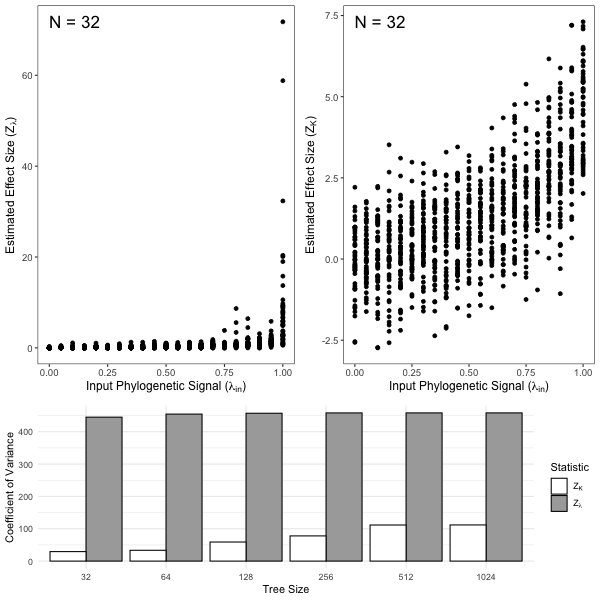
\includegraphics[width=0.95\linewidth]{Fig4}

\singlespacing \textbf{Figure 4}. Variation in estimates of phylogenetic
signal across input levels of phylogenetic signal. (A) Estimates of
Pagel's \(\lambda\) for data simulated on phylogenies with 128 taxa
(\(n=128\)), (B) Estimates of \(Z_K\) for data simulated on phylogenies
with 128 taxa (\(n=128\)), (C) Variance in the variation of
\(\lambda_{est}\) across input levels of phylogenetic signal, estimated
on phylogenies containing differing numbers of species. (D) Variance in
the variation of \(Z_K\) across input levels of phylogenetic signal,
estimated on phylogenies containing differing numbers of species.

\end{document}
